\section{The Git structure}
Git, as it was said before, is a distributed version control system.
It means that each user as a mirror from the repository (local
repository) and in the case of
git, there is no need for a central server, even that, each user is able to
fetch or push updates from other user's repository (remote repository).
Git is divided mainly in three components. The working directory,
the index and the repository. The connection between these components
can be seen in Figure \ref{fig:git_structure}. Local and remote
repository have the same internal structure. What is a local
repository for an user is a remote repository for other user.

\begin{figure}[h!]
   \centering
   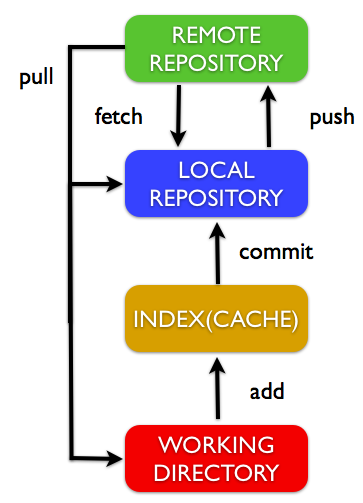
\includegraphics[width=0.8\textwidth]{images/data_flow_simplified.png}
   \caption{Git WorkFlow}\label{fig:git_structure}
\end{figure}

\subsection{Working Directory}

The working directory is basically a subset of
a file system that contains the files of the project you are
currently working on. This files can be the current files, files
retrieved from an old snapshot or even files that are not being
tracked. When retrieving an older snapshot of the project, the
working directory is updated to reflect the project in that state. It
is possible to have in the working directory files that are not being
tracked. This files are just ignored

\subsection{Index}
The index is a component that contains all the files that will be committed
on the next commit (the next snapshot).

\subsection{Repository}
As said, Git is a distributed VCS. So we can work not just with a local repository,
or remote repository, but we can work with both types at the same time. One of 
the advantages of Git is that we can work off-line and then at the end of day,
we update the remote repository with our work. \par
In fact, the definition of local/remote depends only on the perspective of the user,
as there are no structural differences between local and remote repositories. 
Imagining two users, where each one has his local repository, 
one will see the other as the remote repository and vice-versa. \par
A repository contains all the information needed to store, and stores all snapshots taken.
%
%For a matter of time and complexity, in this project we turned our attention 
%mainly to the index and repository. We are not modeling what is going
%on in the working directory. We just model that there are files in the
%working directory, anything else.
